\documentclass{article}

% Overleaf: select FINAL_REPORT.tex as the main document and use pdfLaTeX.
% This report follows the NeurIPS 2026 layout recommended by the DNU Lab.
% Use the preprint option while the report is being edited. Do not use the
% final option unless preparing an accepted NeurIPS camera-ready paper.
\usepackage[preprint]{neurips_2026}

\usepackage[utf8]{inputenc}
\usepackage[T1]{fontenc}
\usepackage{amsmath}
\usepackage{amssymb}
\usepackage{amsfonts}
\usepackage{booktabs}
\usepackage{graphicx}
\usepackage{microtype}
\usepackage{nicefrac}
\usepackage{url}
\usepackage{xcolor}
\usepackage[hidelinks]{hyperref}
\usepackage[capitalize,nameinlink,noabbrev]{cleveref}

% Search the local LaTeX directory first and the Overleaf ZIP layout second.
\graphicspath{{./}{figures/}}
\setlength{\emergencystretch}{2em}

\title{When Does Length-Aware Attention Generalize in a Reduced Binary Classifier?}

\author{%
  Aaron Shin\\
  Dickinson College
}

\begin{document}

\maketitle

\begin{abstract}
Softmax-attention classifiers trained on short sequences can fail to generalize
to much longer ones, even on the simple task of detecting whether a target
token is present, because a single target must compete for a fixed budget of
attention against a crowd of non-target tokens that grows with the sequence.
This report asks when making attention length-aware overcomes that dilution, in
a reduced binary classifier where the mechanism is exactly analyzable: a single
readout query attends over one-hot token embeddings, and because the non-target
tokens are identical, the target's attention mass has an exact closed form. We
compare constant, logarithmic, and learned length scalings, and find one
condition behind all three: to generalize to unbounded length, the scaling must
amplify the target's score margin fast enough to grow faster than the crowd of
non-target tokens. A constant scaling never does; a logarithmic scaling does
when the learned score margin is large enough, and a learned scaling does only
when training makes the amplification fast enough. The consequence is
diagnostic: a model can pass a large finite benchmark, such as ten million
tokens, yet still be predicted to fail at greater lengths, because the quantity
that decides unbounded-length generalization cannot be read off from any single
benchmark.
\end{abstract}

\section{Introduction}
\label{sec:introduction}

Length generalization is a basic difficulty for sequence models. A classifier
can fit short training sequences while relying on a mechanism that does not
remain valid at longer sequence lengths. This problem appears even in simple
existential target-token tasks, where the model only needs to decide whether a
sequence contains a particular token.

The motivating failure mode is attention dilution. Softmax attention divides a
fixed budget of attention among all tokens, so a single target token must
compete with a crowd of non-targets that grows with the sequence; even a fixed
per-token margin for the target can be overwhelmed once that crowd is large
enough. This raises a simple question: can attention be made length-aware,
sharpening as the sequence grows, so that the target keeps enough attention at
long lengths?

This report focuses on a reduced binary classifier for that question. The model
is intentionally much simpler than a full transformer. It uses fixed one-hot
token values, learned query and key projections, a single readout query (the
query at the last position), and a binary classifier. The goal is not to show
that this model is a competitive architecture. The goal is to test whether the
simplified closed-form attention theory correctly describes a trainable model
in the controlled setting where its assumptions can be directly checked.

The reduced model is built so that this theory applies exactly rather than
approximately. Because every non-target token is identical, the attention
scores collapse by construction to just two values, a target score and a shared
non-target score. This two-score structure is precisely what the theory assumes,
and it makes a closed-form expression for the target's attention mass exact,
reducing length generalization to a precise question about how the target's
score margin must grow with length.

The report compares three scaling rules that govern how fast attention sharpens
as the sequence grows: constant, logarithmic, and learned. The experiments play
out as the theory predicts. Constant scaling improves with more training but
always fails eventually. Log scaling succeeds once the score margin the model
learns exceeds 1. Learned-log scaling succeeds at unbounded length only when
optimization drives the product of the learned coefficient and the score
margin above 1. This last regime carries the report's main lesson: a model can
pass a finite benchmark, such as sequences of ten million tokens, yet still be
predicted to fail at larger lengths whenever that product, which the benchmark
alone cannot reveal, stays below 1. Passing a fixed length is therefore not
evidence of unbounded-length generalization; the target's effective margin must
grow faster than the competing crowd.

\section{Related Work}
\label{sec:related-work}

This report describes the output of an independent research project in the Deep
Network Understanding (DNU) Lab of Dickinson College. Consistent with the lab's
emphasis on original research, this report relates its contribution to a small
number of representative works rather than surveying the field comprehensively.
We discuss two such works below, chosen for their direct connection to the
mechanism studied here, and leave a fuller literature review to future work.

The transformer architecture of \citet{vaswani2017attention} places softmax
attention at its center. Each query forms a normalized distribution over the
keys, so a fixed total attention mass is shared among all of them, and the
attention given to any one token depends on how many keys it competes with.
When the number of non-target keys grows with sequence length, this
normalization is exactly the dilution effect studied here. The present report
isolates that effect in a minimal setting where the attention scores and output
values can be read off directly.

\citet{press2022train} study length extrapolation directly and propose attention
with linear biases (ALiBi), which adds a fixed, distance-dependent penalty to
the attention scores so that a model trained on short sequences can be
evaluated on much longer ones. Their method operates in a full transformer and
supplies a recency bias in place of standard positional encodings. The present
report is narrower and more analytical. Rather than proposing a transformer
method, it studies a length-aware multiplier on the scores, an inverse
temperature that may be held fixed or learned, in a reduced classifier where
the condition for length generalization can be derived in closed form and the
learned score geometry can be inspected directly.

\section{Background: Simplified Binary Attention}
\label{sec:background}

This section derives, from the model definition, the score structure and
closed-form target-attention mass previewed in the Introduction, and then uses
that closed form to characterize when the classifier generalizes to unbounded
length.

The task uses a two-token vocabulary:

\begin{description}
  \item[$t$] target token;
  \item[$u$] non-target token.
\end{description}

A positive length-$n$ sequence, with $n\geq2$, contains one target token and
$n-1$ non-target tokens. The token in the last position is always the
non-target token $u$. Because both positive and negative sequences end in $u$,
this position carries no label information; it simply fixes a consistent
readout slot. The model has no positional encoding, so permuting the tokens
among the first $n-1$ positions does not change its output. We place the target
in the first position only to make the notation easier to read; any position
other than the last is equivalent:

\begin{center}
  \texttt{t, u, u, ..., u}
\end{center}

A negative length-$n$ sequence contains only non-target tokens:

\begin{center}
  \texttt{u, u, u, ..., u}
\end{center}

At a high level, the query at the last position (the readout query) scores every
token in the sequence, softmax converts those scores into attention weights,
and the weighted sum of the token values is passed to a binary classifier.

The model begins with fixed one-hot embeddings for $t$ and $u$:

\begin{equation}
  t \mapsto [1,0],
  \qquad
  u \mapsto [0,1].
  \label{eq:token-embeddings}
\end{equation}

A length-$n$ sequence is thus represented by a one-hot matrix
$X\in\mathbb{R}^{n\times2}$ with one token embedding per row. The learned query
and key projections are $Q=XW_Q$ and $K=XW_K$ with
$W_Q,W_K\in\mathbb{R}^{2\times d}$, so $Q,K\in\mathbb{R}^{n\times d}$ and
$q_{\mathrm{last}}$ is the last row of $Q$. Here $d$ is the query and key
dimension, set to $d=2$ throughout. Conventional self-attention forms the full
$n\times n$ score matrix $QK^\top/\sqrt{d}$. This reduced classifier uses only
the query at the last position and therefore needs only its scores against the
$n$ keys:

\begin{equation}
  s_j=\frac{q_{\mathrm{last}}^\top k_j}{\sqrt{d}},
  \qquad j=1,\ldots,n.
  \label{eq:reduced-score}
\end{equation}

Since the token in the last position is $u$, $q_{\mathrm{last}}=q_u$ for every
example. Writing $k_t$ and $k_u$ for the target and non-target keys, which are
position-independent, the target and non-target scores, and the score margin
between them, are

\begin{equation}
  a=\frac{q_u^\top k_t}{\sqrt{d}},
  \qquad
  b=\frac{q_u^\top k_u}{\sqrt{d}},
  \qquad
  \Delta=a-b.
  \label{eq:target-nontarget-scores}
\end{equation}

The architecture thus fixes the score vector of a positive example to the
two-score structure

\begin{equation}
  S_n=(a,b,b,\ldots,b),
  \label{eq:two-score-structure}
\end{equation}

while training determines only the two values $a$ and $b$. Because there is a
single non-target type, every non-target position holds the same token, hence
the same key and the same score $b$ by construction.

The central change in this study is an additional score multiplier $\alpha(n)$
applied before softmax. The attention weight on position $j$ is

\begin{equation}
  A_j
  =
  \frac{e^{\alpha(n)s_j}}
       {\sum_{i=1}^{n}e^{\alpha(n)s_i}}.
  \label{eq:attention-weight}
\end{equation}

Since $\alpha(n)$ multiplies the scores inside the softmax, it acts as a
length-dependent inverse temperature: larger $\alpha(n)$ sharpens the
attention. Standard attention corresponds to $\alpha(n)=1$. The length-aware
variants instead make $\alpha(n)$ grow with the sequence length. We consider
three choices of $\alpha(n)$: constant, logarithmic, and learned logarithmic.
Each is analyzed in turn below.

For the positive score vector $S_n=(a,b,\ldots,b)$, the attention mass on the
single target key is

\begin{equation}
  p_t(n)
  =
  \frac{e^{\alpha(n)a}}
       {e^{\alpha(n)a}+(n-1)e^{\alpha(n)b}}
  =
  \frac{e^{\alpha(n)\Delta}}
       {e^{\alpha(n)\Delta}+(n-1)},
  \label{eq:target-attention}
\end{equation}

where the second form follows by dividing the numerator and denominator by
$e^{\alpha(n)b}$.

The value pathway reuses these one-hot embeddings directly as value vectors,
with no learned value projection, so the value vector $v_j$ at position $j$ is
$[1,0]$ when its token is the target and $[0,1]$ otherwise. This makes the
output directly record how much total attention is assigned to each token type.
The classifier reads the weighted sum of these value vectors:

\begin{equation}
  o(n)=\sum_{j=1}^{n}A_jv_j.
  \label{eq:attention-output}
\end{equation}

On a positive example, the target carries weight $p_t(n)$ and the non-targets
together carry the remaining $1-p_t(n)$, so the output is a convex combination
of the two value vectors:

\begin{align}
  o_{\text{pos}}(n)
  &=p_t(n)[1,0]+\bigl(1-p_t(n)\bigr)[0,1]
  \nonumber\\
  &=\bigl(p_t(n),1-p_t(n)\bigr).
  \label{eq:positive-output}
\end{align}

A negative example contains only $u$, so its output is always

\begin{equation}
  o_{\text{neg}}(n)=[0,1].
  \label{eq:negative-output}
\end{equation}

The negative output is this same combination with target mass 0, so both
outputs are fixed by the single scalar $p_t(n)$. A learned linear layer reads
this output, so on a positive example the classifier produces the logit

\begin{align}
  z(n)
  &=w_t p_t(n)+w_u\bigl(1-p_t(n)\bigr)+\beta
  \nonumber\\
  &=(w_t-w_u)p_t(n)+(w_u+\beta),
  \label{eq:classifier-logit}
\end{align}

with learned weights $w_t,w_u$ and bias $\beta$, and predicts target-present
when $z(n)\geq0$. Since the slope $w_t-w_u$ is positive in the trained model,
the logit increases with $p_t(n)$, so classification reduces to a threshold:
the model predicts target-present when $p_t(n)\geq p^{\ast}$, with
$p^{\ast}=-(w_u+\beta)/(w_t-w_u)$. If $p_t(n)\to0$, the positive
representation converges to the negative representation, and the
representation gap between the two classes vanishes. If $p_t(n)$ converges to a
constant strictly between 0 and 1, classification depends on this threshold.
The stronger, target-dominant outcome is $p_t(n)\to1$. The conditions below
distinguish these three cases.

\subsection{Length-Scaling Regimes}
\label{sec:length-scaling-regimes}

Assume that $\Delta>0$, so the target has a score advantage over each
non-target. If $\Delta\leq0$, none of the multipliers considered below can
create such an advantage, since each $\alpha(n)$ is positive and scales
$\Delta$ without changing its sign. The competing term $(n-1)$ is the source
of length dependence: it grows like $n$, so the target term
$e^{\alpha(n)\Delta}$ must grow at least as fast for target attention to
survive. A logarithmic $\alpha(n)$ is the natural way to achieve this, since it
turns $e^{\alpha(n)\Delta}$ into a power of $n$.

For the constant baseline $\alpha(n)=1$,

\begin{equation}
  p_t(n)
  =
  \frac{e^\Delta}{e^\Delta+(n-1)}
  \longrightarrow 0
  \qquad\text{as }n\to\infty.
  \label{eq:constant-limit}
\end{equation}

A fixed score margin can beat each non-target token individually, but it cannot
beat an unbounded number of non-target competitors. Consequently,
$o_{\text{pos}}(n)\to[0,1]$, the same representation as
$o_{\text{neg}}(n)$.

For the log multiplier $\alpha(n)=\log n$, we have
$e^{\alpha(n)\Delta}=e^{\Delta\log n}=n^\Delta$, so

\begin{equation}
  p_t(n)
  =
  \frac{n^\Delta}{n^\Delta+n-1}.
  \label{eq:log-attention}
\end{equation}

The limit depends on the score margin:

\begin{equation}
  \lim_{n\to\infty}p_t(n)
  =
  \begin{cases}
    1, & \Delta>1,\\
    \tfrac12, & \Delta=1,\\
    0, & 0<\Delta<1.
  \end{cases}
  \label{eq:log-limit}
\end{equation}

Thus $\Delta>1$ makes target attention converge to 1, while $0<\Delta<1$
causes the positive representation to collapse onto the negative
representation. At the boundary $\Delta=1$, the two representations remain
distinct, and classification depends on the learned decision boundary.

For the learned-log multiplier used in the experiments,

\begin{equation}
  \alpha(n)=1+c\log(1+n),
  \label{eq:learned-log-multiplier}
\end{equation}

where $c$ is a learned, strictly positive coefficient. The additive 1 makes
$\alpha=1$ at $c=0$, recovering the constant baseline, and using $\log(1+n)$
keeps the multiplier well-defined at small $n$; neither term changes the
asymptotic exponent, which is governed by $c\Delta$. Since
$e^{\alpha(n)\Delta}=e^\Delta(1+n)^{c\Delta}$, the target attention mass is

\begin{equation}
  p_t(n)
  =
  \frac{e^\Delta(1+n)^{c\Delta}}
       {e^\Delta(1+n)^{c\Delta}+(n-1)}.
  \label{eq:learned-log-attention}
\end{equation}

Its limit is

\begin{equation}
  \lim_{n\to\infty}p_t(n)
  =
  \begin{cases}
    1, & c\Delta>1,\\
    \dfrac{e^\Delta}{e^\Delta+1}, & c\Delta=1,\\
    0, & c\Delta<1.
  \end{cases}
  \label{eq:learned-log-limit}
\end{equation}

Thus $c\Delta>1$ makes target attention converge to 1. The equality case again
has a nonzero limiting target mass and depends on the classifier's decision
boundary, whereas $c\Delta<1$ produces asymptotic collapse.

A single condition unifies all three regimes. Writing the target attention mass
as

\begin{equation}
  p_t(n)
  =
  \frac{1}{1+\exp\!\left(\log(n-1)-\alpha(n)\Delta\right)}
  =\sigma\bigl(g(n)\bigr),
  \qquad
  g(n)=\alpha(n)\Delta-\log(n-1),
  \label{eq:general-gap}
\end{equation}

with $\sigma$ the sigmoid function, target attention converges to 1 exactly
when $g(n)\to+\infty$, that is, when the effective margin
$\alpha(n)\Delta$ outgrows $\log(n-1)$ without bound. Since $\log(n-1)$ grows
like $\log n$ with coefficient 1, the outcome is decided by how fast
$\alpha(n)\Delta$ grows: it stays bounded for the constant baseline, so target
attention always collapses, and grows like $\Delta\log n$ for the log
multiplier and $c\Delta\log n$ for the learned-log multiplier. Target dominance
therefore needs the coefficient of $\log n$ to exceed 1, giving the thresholds
$\Delta>1$ and $c\Delta>1$. This is the precise sense in which length
generalization requires the effective margin to grow faster than the logarithm
of the number of competing non-target keys.

\section{Experimental Design}
\label{sec:experimental-design}

The experiments train the reduced model derived above (fixed one-hot embeddings
reused as value vectors, learned query and key projections
$W_Q,W_K\in\mathbb{R}^{2\times2}$, a readout query, softmax attention, and a
binary classifier on the two-dimensional attention output) and vary the score
multiplier $\alpha(n)$ across three modes:

\begin{center}
  \begin{tabular}{ll}
    \toprule
    Mode & $\alpha(n)$ \\
    \midrule
    \texttt{constant} & $1$ \\
    \texttt{log} & $\log n$ \\
    \texttt{learned\_log} & $1+c\log(1+n)$ \\
    \bottomrule
  \end{tabular}
\end{center}

For \texttt{learned\_log}, the coefficient is
$c=\operatorname{softplus}(k_\alpha)$, where $k_\alpha$ is an unconstrained
learnable scalar, so $c$ stays positive during optimization.

The classifier maps the attention output to the logit $z(n)$ introduced above;
an example is classified target-present when $z(n)\geq0$, equivalently when
its sigmoid probability is at least 0.5. Two quantities from the classifier
appear in the results: the positive-example logit, the value of $z(n)$ on a
positive example, whose sign decides whether that example is classified
correctly; and the positive-example accuracy (equivalently, recall), the
fraction of positive examples with $z(n)\geq0$.

Each run trains at length 10 on 2,000 examples split evenly between positive
and negative, minimizing binary cross-entropy on the logit with AdamW (learning
rate $3\times10^{-3}$, no weight decay, batch size 64). One epoch is a single
pass over the 2,000 examples, or 32 optimizer steps. Each configuration is
trained under five random seeds (0--4), and all reported numbers are the mean
and standard deviation across these seeds.

Each trained model is evaluated at the seven powers of ten from $10$ to
$10^7$, six orders of magnitude beyond the training length, on 50 balanced
examples per length. Because a length-$10^7$ evaluation cannot be held in
memory at once, examples are generated and scored in small chunks, so the full
evaluation tensor is never materialized.

Each run is labeled by its multiplier mode and epoch budget: for example,
\texttt{constant\_e50} is constant scaling trained for 50 epochs.
\Cref{tab:main-results} lists all eight runs: constant at 50, 100, and 1,000
epochs; log at 50; and learned-log at 50, 100, 200, and 400.
\Cref{fig:attention-and-logit} shows six of them, keeping every constant budget
and the two learned-log budgets that bracket the $c\Delta=1$ threshold; the
omitted \texttt{learned\_log\_e100} and \texttt{learned\_log\_e400} fall on
the same sides.

\section{Results}
\label{sec:results}

In this task, length generalization is decided entirely by the positive
examples. A negative sequence contains only non-target values, so its attention
output is exactly the non-target representation $[0,1]$ by construction,
independent of how attention is spread; because the learned threshold satisfies
$p^{\ast}>0$ in every run, negatives are classified correctly at every length.
The difficulty lives in the positive examples: the target mass $p_t$ can dilute
with length until the classifier no longer detects the target.
\Cref{tab:main-results} reports each run at $10^7$, and
\cref{fig:attention-and-logit} traces the target mass $p_t$ in panel (a) and
the positive-example logit in panel (b).

\begin{table}[t]
  \caption{Main results at $n=10^7$, as means over five seeds ($\pm$ one
  standard deviation). The $p_t$, logit, and accuracy columns are measured on
  positive examples; negative accuracy is 100\% in every run.}
  \label{tab:main-results}
  \centering
  \small
  \setlength{\tabcolsep}{2.5pt}
  \resizebox{\linewidth}{!}{%
  \begin{tabular}{lrrrrrrr}
    \toprule
    Run & Steps & $\Delta$ & $c$ & $c\Delta$ & $p_t$ & Logit & Accuracy \\
    \midrule
    \texttt{constant\_e50} & 1,600 & $9.0\pm0.2$ & n/a & n/a &
      $0.001\pm0.000$ & $-3.3\pm0.1$ & 0\% \\
    \texttt{constant\_e100} & 3,200 & $9.9\pm0.2$ & n/a & n/a &
      $0.002\pm0.000$ & $-4.5\pm0.1$ & 0\% \\
    \texttt{constant\_e1000} & 32,000 & $13.2\pm0.2$ & n/a & n/a &
      $0.050\pm0.010$ & $-17.3\pm0.4$ & 0\% \\
    \texttt{log\_e50} & 1,600 & $4.4\pm0.1$ & n/a & n/a &
      $1.000\pm0.000$ & $3.2\pm0.1$ & 100\% \\
    \texttt{learned\_log\_e50} & 1,600 & $8.1\pm0.2$ & $0.072\pm0.006$ &
      $0.58\pm0.03$ & $0.788\pm0.075$ & $1.9\pm0.5$ & 100\% \\
    \texttt{learned\_log\_e100} & 3,200 & $8.6\pm0.3$ & $0.096\pm0.008$ &
      $0.83\pm0.05$ & $0.997\pm0.002$ & $4.6\pm0.1$ & 100\% \\
    \texttt{learned\_log\_e200} & 6,400 & $9.0\pm0.3$ & $0.126\pm0.010$ &
      $1.14\pm0.06$ & $1.000\pm0.000$ & $6.4\pm0.1$ & 100\% \\
    \texttt{learned\_log\_e400} & 12,800 & $9.4\pm0.3$ & $0.166\pm0.013$ &
      $1.55\pm0.08$ & $1.000\pm0.000$ & $9.6\pm0.1$ & 100\% \\
    \bottomrule
  \end{tabular}
  }
\end{table}

\begin{figure}[t]
  \centering
  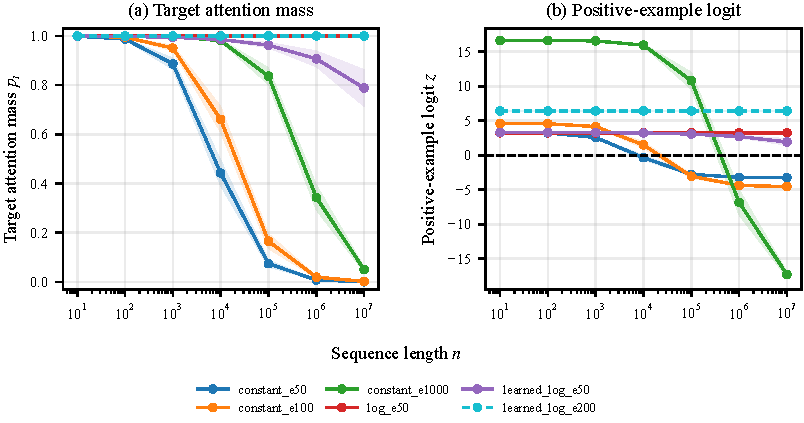
\includegraphics[width=\linewidth]{final_report_attention_and_logit_by_length.pdf}
  \caption{Target attention mass and positive-example logit versus sequence
  length for six representative runs (mean over five seeds; shaded bands show
  $\pm1$ s.d.). (a) Runs that generalize saturate at $p_t=1$, so
  \texttt{log\_e50} and \texttt{learned\_log\_e200} overlap, with the latter
  dashed. (b) The logit curves distinguish these overlapping runs; the
  horizontal dashed line at $z=0$ marks the decision boundary.}
  \label{fig:attention-and-logit}
\end{figure}

\subsection{Constant Scaling}

Constant scaling uses $\alpha=1$. At any fixed $\Delta$ this gives
$p_t(n)\to0$. Empirically, more training increases $\Delta$, moving the
failure point outward without changing this asymptotic regime: the
positive-example accuracy at $10^7$ is 0 for all three budgets in every seed.
More training even drives the positive-example logit more negative, not less
(\cref{tab:main-results}: $-3.3$, $-4.5$, and $-17.3$ for e50, e100, and
e1000): once the target mass has collapsed, the logit is set by the learned
intercept $w_u+\beta$, which itself grows more negative with training. The
larger margin only postpones the collapse; the theory still predicts failure
for any finite fixed margin.

\subsection{Log Scaling}

Log scaling uses $\alpha=\log n$. The score margin is
$\Delta=4.4\pm0.1$, comfortably above the threshold $\Delta>1$ in every seed,
so the theory predicts $p_t(n)\to1$, which is what is observed: target attention
reaches 1.000 at long lengths, the positive-example logit stays positive, and
the positive-example accuracy is 1 at $10^7$ in all five seeds.

\subsection{Learned Log Scaling}

Learned-log scaling uses $\alpha=1+c\log(1+n)$. These runs separate
finite-length success from asymptotic success. At 50 and 100 epochs the model
already passes the $10^7$ benchmark, with positive-example accuracy 1 in all
five seeds, yet the product $c\Delta$ stays below the threshold,
$0.58\pm0.03$ and $0.83\pm0.05$, respectively, so the theory predicts eventual
failure at larger lengths. Solving the closed-form $p_t(n)$ for the length at
which target attention drops to the classifier's per-seed decision threshold
$p^{\ast}$ quantifies this (derivation in Appendix~A): across
seeds, the 50-epoch runs ($c\Delta\approx0.58$) are predicted to fail near
$n\sim10^8$--$10^9$, within about two orders of magnitude of the benchmark. The
100-epoch runs ($c\Delta\approx0.83$) are pushed beyond $n\sim10^{18}$, the
failure length climbing steeply as $c\Delta\to1$.

Only at 200 epochs does $c\Delta$ exceed 1 in every seed
($1.14\pm0.06$), entering the asymptotic-success regime; by 400 epochs it is
well clear ($1.55\pm0.08$). The crossing is driven by the coefficient $c$,
which grows monotonically with the training budget
($0.072\to0.096\to0.126\to0.166$) while the score margin $\Delta$ grows only
modestly ($8.1\to8.6\to9.0\to9.4$).

The e50 and e100 budgets reach 100\% at $10^7$ with $c\Delta<1$: passing at one
length does not certify generalization to every length. The property that
transfers is $c\Delta>1$, not accuracy at any single point.
\Cref{tab:main-results} shows this directly: \texttt{constant\_e50} and
\texttt{learned\_log\_e200} learn the same score margin ($\Delta=9.0$), yet the
first collapses ($p_t=0.001$, 0\%) and the second saturates ($p_t=1.000$,
100\%). The difference comes from the length scaling, not from $\Delta$.

\section{Mechanism: What the Model Learns}
\label{sec:mechanism}

The reduced model also allows a direct weight-level explanation of where
$\Delta$ comes from. Recall that the readout query is $q_u$ (the last token is
always the non-target $u$), the target key is $k_t$, and the non-target key is
$k_u$. The target and non-target scores are then

\begin{equation}
  a=\frac{q_u^\top k_t}{\sqrt{d}},
  \qquad
  b=\frac{q_u^\top k_u}{\sqrt{d}}.
  \label{eq:mechanism-scores}
\end{equation}

The score margin is therefore

\begin{equation}
  \Delta
  =a-b
  =\frac{q_u^\top(k_t-k_u)}{\sqrt{d}}.
  \label{eq:mechanism-margin}
\end{equation}

For one \texttt{learned\_log\_e200} checkpoint (seed 1), the learned vectors
are approximately

\begin{equation}
  q_u=
  \begin{bmatrix}
    -1.830\\
     1.646
  \end{bmatrix},
  \qquad
  k_t=
  \begin{bmatrix}
    -2.232\\
     1.642
  \end{bmatrix},
  \qquad
  k_u=
  \begin{bmatrix}
     1.990\\
    -1.428
  \end{bmatrix}.
  \label{eq:learned-vectors}
\end{equation}

With $d=2$, this gives

\begin{equation}
  a\approx4.799,
  \qquad
  b\approx-4.237,
  \qquad
  \Delta\approx9.036.
  \label{eq:mechanism-values}
\end{equation}

\begin{figure}[t]
  \centering
  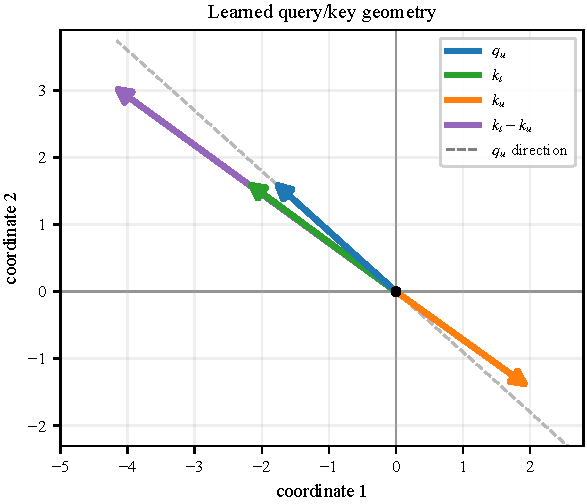
\includegraphics[width=0.68\linewidth]{final_report_mechanism_vectors.pdf}
  \caption{Learned query and key vectors for
  \texttt{learned\_log\_e200} (seed 1), drawn in the $d=2$ query/key space.}
  \label{fig:mechanism-vectors}
\end{figure}

Geometrically (\cref{fig:mechanism-vectors}), $q_u$ points in a direction that
separates the target key from the non-target key. The target key has a positive
projection along the readout query direction, while the non-target key has a
negative projection. Equivalently, $q_u$ aligns with the difference vector
$k_t-k_u$. This alignment creates the score pattern $a>b$, the positive score
margin $\Delta$ that the length-scaling analysis assumes.

The geometry is the same in every seed: across seeds 0--4 the target score $a$
is positive and the non-target score $b$ negative, $q_u$ is nearly collinear
with $k_t-k_u$ (cosine $\geq0.99$), and $\Delta=9.03\pm0.28$.

This mechanism explains how the model creates a target advantage, but it also
shows why a target advantage is not by itself enough. Under constant scaling,
even a large fixed $\Delta$ is eventually overwhelmed by the growing number of
non-target positions. Learned-log attention has an additional degree of
freedom: it can increase the coefficient $c$ so that the effective margin grows
like $c\Delta\log n$. In the successful learned-log run, optimization makes the
product $c\Delta$ cross the threshold.

\section{Discussion}
\label{sec:discussion}

The main contribution of this report is a controlled analysis of length-aware
attention scaling in a trainable reduced model. The two-token,
position-independent construction makes the two-score structure expected by
design; it is not itself a learned discovery. This simplification lets us apply
the closed-form target-attention equation directly and isolate the effect of
the score multiplier from other transformer components.

The result also sharpens the distinction between finite and asymptotic
generalization. A run can clear a fixed length such as $10^7$ while $c\Delta$
still sits below 1, so passing a benchmark certifies only finite-length
behavior, not the limit. What survives to unbounded length is a structural
property of the learned solution, $c\Delta>1$, and exposing that property
cleanly, rather than a single-length benchmark score, is what the reduced model
is for.

The reduced model is intentionally limited. It uses fixed semantic value
vectors, no positional encodings, one readout query, and a simple binary
classifier. These restrictions make the mechanism easy to analyze, but they
also mean the conclusion should not be transferred directly to a full
transformer, which can have non-identical non-target scores, learned value
vectors, multiple heads, residual streams, feed-forward layers, layer
normalization, and pooling. Any of these can break the exact two-score structure
the analysis relies on.

The value of the reduced model is therefore diagnostic. It separates two
questions that are entangled in a full transformer. First, can the architecture
create a score margin $\Delta$? Second, does the length-scaling mechanism make
the effective margin grow fast enough to beat the softmax denominator? In this
controlled binary setting, the answer to both questions can be measured
directly.

Two directions follow. The first is to relax these restrictions toward a full
transformer and test whether an analog of the $c\Delta>1$ condition still
governs length generalization once non-identical non-target scores, learned
values, and depth are reintroduced. The second is to move beyond binary
detection to broader versions of the task, such as identifying which target
type is present or counting how many targets occur.

\section{Conclusion}
\label{sec:conclusion}

This report studied length generalization in a reduced binary attention
classifier whose two-score structure makes the closed-form target-attention
expression exact.

Across the three scaling rules, the experiments give a consistent picture:
constant scaling fails at any sufficiently large length, while log and
learned-log scaling generalize only when their effective margin outgrows the
competing crowd, requiring $\Delta>1$ and $c\Delta>1$, respectively. In this
reduced setting, then, the central condition for length generalization is not
fitting the training length or passing a finite long-length benchmark; the
effective margin must grow faster than the logarithm of the number of competing
non-target keys.

\clearpage
\appendix

\section{Supporting Material}
\label{app:supporting-material}

\subsection{Learned Query and Key Matrices for the Mechanism Example}
\label{app:mechanism-matrices}

The Mechanism section reports the query and key vectors of
\texttt{learned\_log\_e200} (seed 1). They come from the two learned projection
matrices, which for that run are

\begin{equation}
  W_Q=
  \begin{pmatrix}
     0.364 & -0.137\\
    -1.830 &  1.646
  \end{pmatrix},
  \qquad
  W_K=
  \begin{pmatrix}
    -2.232 &  1.642\\
     1.990 & -1.428
  \end{pmatrix}.
  \label{eq:learned-projection-matrices}
\end{equation}

Because the token embeddings are one-hot, with $t\mapsto[1,0]$ and
$u\mapsto[0,1]$, each token's query and key is the corresponding row: the first
row gives $q_t$ and $k_t$, and the second gives $q_u$ and $k_u$. This recovers
the vectors and scores reported in the Mechanism section.

Two details are worth recording. The readout query is always $q_u$, because the
last token is always the non-target $u$, so the first row of $W_Q$ is never used
by the model; it stays near its initialization at
$q_t=(0.364,-0.137)$. The matrices are also not individually identifiable: the
model depends on them only through the product $W_QW_K^\top$, whose entries
divided by $\sqrt{d}$ are the scores, so any other pair with the same product
defines exactly the same model. The invariant content is the scores, not the
individual entries.

\subsection{Predicted Learned-Log Failure Lengths}
\label{app:failure-lengths}

For a learned-log run with $c\Delta<1$, the target attention decays to zero, so
a positive example is misclassified once $p_t(n)$ falls to the classifier's
decision threshold $p^{\ast}=-(w_u+\beta)/(w_t-w_u)$. We call the length at
which this happens the failure length $n^{\ast}$, defined by
$p_t(n^{\ast})=p^{\ast}$. In every learned-log run the trained threshold sits
close to one half ($p^{\ast}\approx0.497$), so $n^{\ast}$ is essentially the
length at which the target loses the majority of the attention.

Substituting the learned-log closed form
$p_t(n)=e^{\Delta}(1+n)^{c\Delta}/\bigl(e^{\Delta}(1+n)^{c\Delta}+(n-1)\bigr)$
and rearranging gives

\begin{equation}
  \frac{n-1}{(1+n)^{c\Delta}}
  =
  e^{\Delta}\frac{1-p^{\ast}}{p^{\ast}}.
  \label{eq:failure-length-identity}
\end{equation}

At the lengths of interest, $n-1\approx n$ and $1+n\approx n$, so

\begin{equation}
  n^{\ast}
  \approx
  \left(
    e^{\Delta}\frac{1-p^{\ast}}{p^{\ast}}
  \right)^{1/(1-c\Delta)}.
  \label{eq:failure-length-approximation}
\end{equation}

The exponent $1/(1-c\Delta)$ is the important term. It diverges as
$c\Delta\to1$, so a small change in $c\Delta$ near the threshold moves
$n^{\ast}$ by many orders of magnitude.

Evaluating this per seed, using each run's own $\Delta$, $c$, and $p^{\ast}$,
gives failure lengths of $10^{7.7}$ to $10^{9.2}$ for
\texttt{learned\_log\_e50} ($c\Delta\approx0.58$) and $10^{17.8}$ to
$10^{34.4}$ for \texttt{learned\_log\_e100} ($c\Delta\approx0.83$). Both
budgets clear the $10^7$ benchmark, but the 50-epoch runs are predicted to fail
within about two orders of magnitude of it, while the 100-epoch runs fail only
far beyond it. The approximation above agrees with a direct numerical solve of
$p_t(n^{\ast})=p^{\ast}$ to the precision shown.

\section*{Use of Artificial Intelligence}

AI assistants were used throughout this project. They wrote most of the
experiment code, including the model and the training loop. They organized the
run data into a readable form and assisted the analysis that produced the
diagnostics behind \cref{tab:main-results}, the failure-length prediction in
Appendix~A, and the figures. They also drafted and revised the
report prose.

The direction of the work was human throughout. The author ran the experiments,
derived the closed-form analysis and the $c\Delta>1$ condition, chose the
questions, directed the AI's work at every step, and made the judgment calls
that shaped the report. The reduced model was proposed by the project advisor,
who also reviewed the manuscript and set the scope of the main text. Every
reported number was checked against the run data, and the author is responsible
for all claims made here.

\bibliographystyle{plainnat}
\bibliography{references}

% The DNU Lab report does not require the NeurIPS checklist.

\end{document}
